\documentclass{article}
\usepackage{graphicx} % Para insertar imágenes
\usepackage[utf8]{inputenc} % Para caracteres especiales
\usepackage{geometry} % Para ajustar márgenes
\geometry{a4paper, margin=1in} % Configuración de márgenes

\title{
    \textbf{Universidad Católica de Salta} \\
    \vspace{0.5cm}
    \textbf{Ingeniería en Informática} \\
    \vspace{0.5cm}
    \textbf{Cátedra: Lenguaje III} \\
    \vspace{0.5cm}
    \textbf{Docente: Nancy Lucero – Ing. Alejandro Delgado} \\
    \vspace{1cm}
    \textbf{Trabajo Práctico N°1}
}
\author{Nicolás Robledo}
\date{Marzo 2025}

\begin{document}

\maketitle

\section{Introducción}

En este trabajo práctico se diseñó una página web utilizando HTML y CSS. A continuación, se presenta la captura de pantalla de la página web desarrollada.

\section{Captura de pantalla}

\begin{figure}[h]
    \centering
    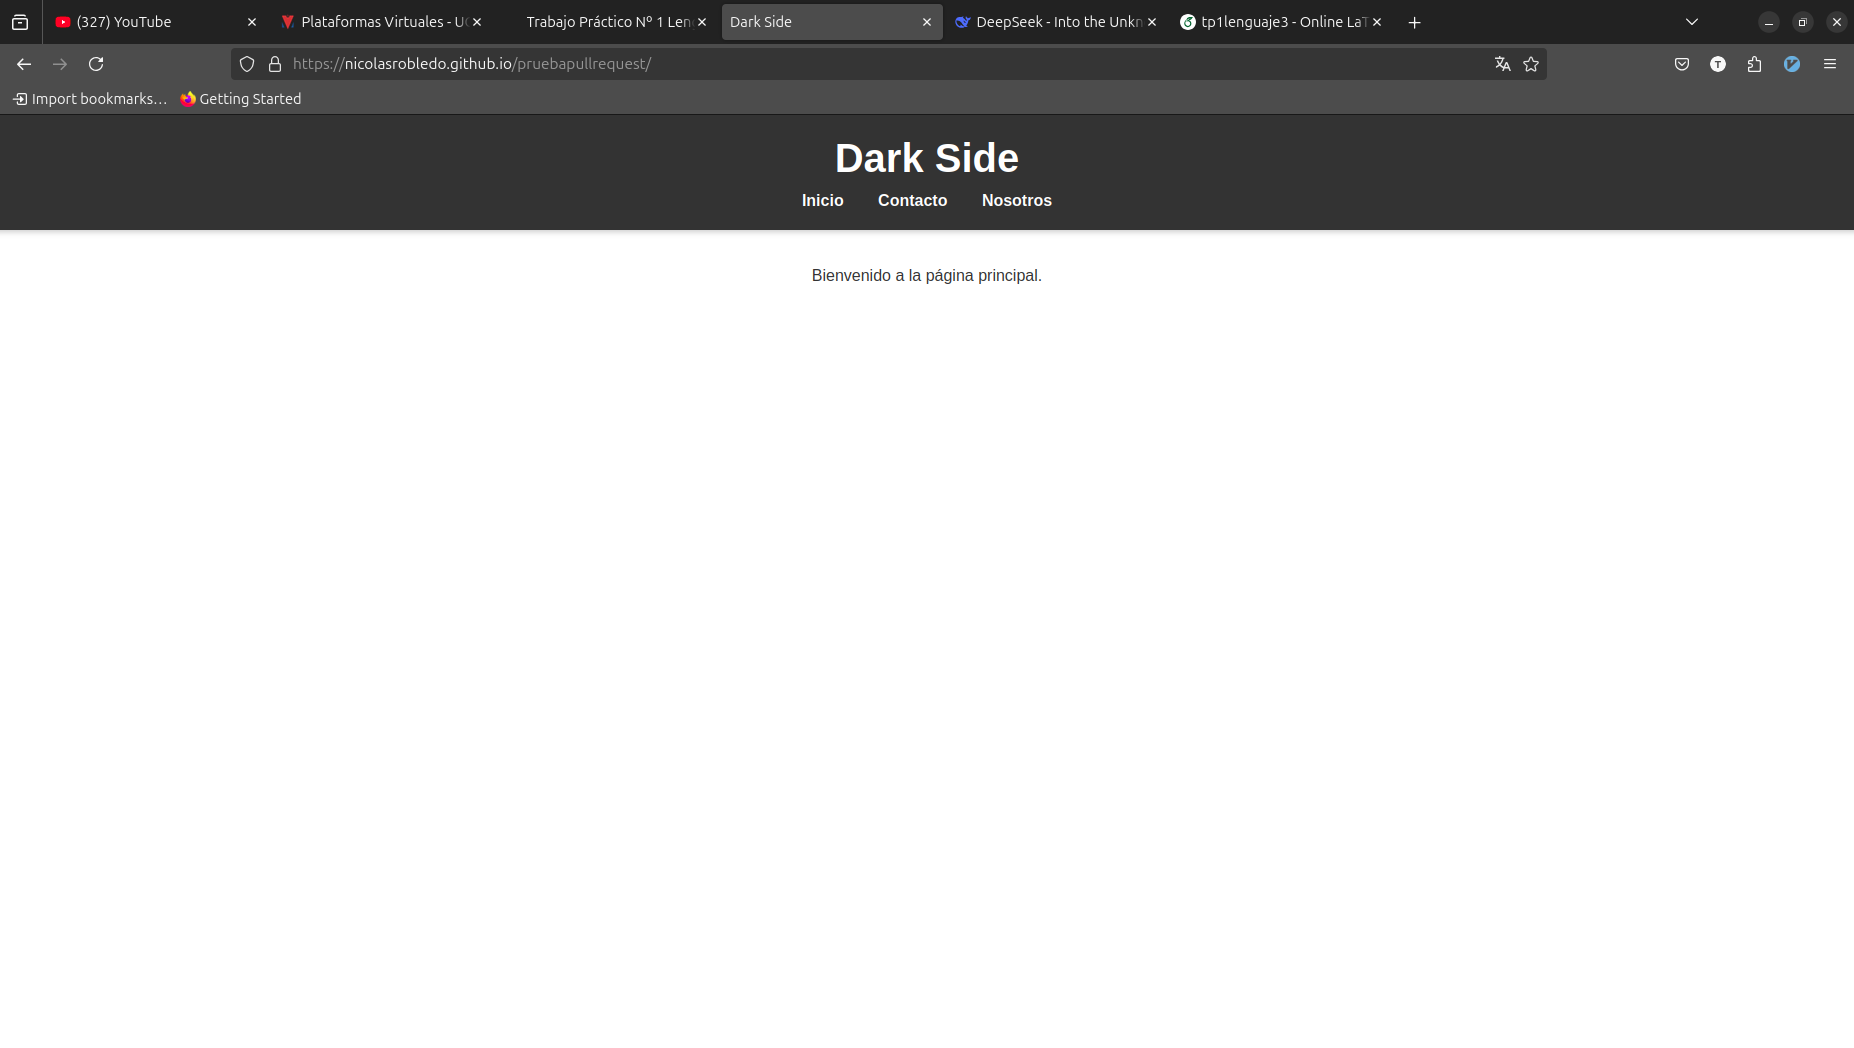
\includegraphics[width=0.9\textwidth]{Pasted image.png} % Reemplaza "captura.png" con el nombre de tu archivo
    \caption{Captura de pantalla de la página web: \url{https://nicolasrobledo.github.io/pruebapullrequest/}}
    \label{fig:captura}
\end{figure}

\end{document}
